\chapter{刘维尔定理与哈密顿流}

\lectureoverview{哈密顿方程所做的远不止重新包装运动方程。它们在相空间上定义了一个散度为零的速度场。这一简单的相消就是刘维尔定理：哈密顿演化保持相空间体积。我们将按照其含义逐渐显现的顺序来达到它---首先是能量守恒，然后是等能面，接着是可能初始条件构成的流体，最后是保体积流与耗散汇之间的对比。同样的语言自然地引向泊松括号。}

\section{为什么还需要另一种形式的力学？}

我们要寻求的定理，是课程开头引入的可逆状态图的连续经典对应物。在可逆的离散定律中，每个状态都有一条箭头进入、一条箭头离开。现在足以确定下一个状态和先前的状态。坏的定律把许多状态送入一个汇：未来或许可以确定，但过去不再可恢复。

刘维尔定理说明了当状态集合是连续相空间时，这一区别会变成什么。取代“一进一出”的说法将是\emph{流入与流出一样多}。然而，在这一说法能够被数学化之前，我们需要从哈密顿方程重构出流。

这样做有一个历史谜题。哈密顿、雅可比、拉格朗日和泊松构建了精巧而优美的经典力学形式，却并不知道量子理论会使这些形式变得不可或缺。牛顿有一个直接的目标：行星运动。拉格朗日和哈密顿面前也有物理问题，但他们追求的类比和结构远远超出任何单一轨道。力学中的稳定作用量类似于光学中的最短时间原理；光线运动和粒子运动可以被纳入平行的数学形式。他们简化、重新排列并统一了方程，因为这些结构本身似乎就包含着物理。

我们现在知道，这种直觉具有非凡的生产力。从逻辑上讲，经典力学的许多特征可以理解为量子力学的极限。从历史上看，顺序是相反的：经典结构先被发现，很久以后它们的深层用途才变得清晰。一则归于费曼的挑衅性笑话通过对比数学的内部追求与受外部伙伴——物理世界——约束的物理学，点明了这一点。这个笑话不是论证，但这一区分是有用的：形式美在这里很重要，因为自然反复选择这些形式结构。

\begin{classroomqa}
  \audiencequestion{牛顿是否具有现代的动能概念，能量的概念又始于何处？
  \lecturetimestamp{00:04:24--00:05:50}}
  \lecturerresponse{牛顿的力学围绕力和运动组织，而不是围绕成熟的普遍能量原理。确切的历史优先次序在讨论中并未定论。莱布尼茨的\emph{活力}，\(\sum_i m_i v_i^2\)，是一个重要的前身，等于现代动能的两倍。后来关于热的研究使热与机械功之间的转换成为核心。早期的热质说把热视为一种守恒的物质，因此能量形式可相互转换的现代观念只是逐渐出现的。}
\end{classroomqa}

\section{哈密顿方程与能量守恒}

设一个系统有\(n\)对正则变量，
\begin{equation}
  (q_i,p_i),\qquad i=1,\ldots,n.
  \label{eq:l7-canonical-pairs}
\end{equation}
每个坐标有一个动量，每个动量有一个坐标。运动定律被封装在一个函数中，
\begin{equation}
  H=H(q_1,\ldots,q_n,p_1,\ldots,p_n,t),
  \label{eq:l7-hamiltonian}
\end{equation}
而哈密顿方程为
\begin{equation}
  \boxed{
  \dot q_i=\frac{\partial H}{\partial p_i},
  \qquad
  \dot p_i=-\frac{\partial H}{\partial q_i}.}
  \label{eq:l7-hamilton-equations}
\end{equation}
符号是正则结构的一部分。\(q\)方程带正号；\(p\)方程带负号。

\begin{figure}[htbp]
  \centering
  \includegraphics[width=0.82\textwidth]{lecture_07_figure_02.png}
  \caption{正则变量、函数\(H(q,p)\)，以及回顾开头处的动量侧哈密顿方程。}
  \lectureframe{00:07:29}
\end{figure}

尽管方程以带指标的对出现，动力学不必逐对分离。哈密顿量可以耦合每一个\(q_i\)和\(p_i\)，因此例如\(\dot p_1\)可能依赖于整个系统的状态。

\begin{classroomqa}
  \audiencequestion{现在的表述是公理化的吗？\(p\)与\(q\)之间假定了什么关系？
  \lecturetimestamp{00:17:08--00:18:18}}
  \lecturerresponse{一旦指定了\(H(q,p)\)和正则对，哈密顿方程就定义了形式理论。不存在普遍的额外假设\(p=m\dot q\)。该关系对具有二次动能的普通笛卡尔粒子成立，但其他坐标和其他哈密顿量给出其他动量--速度关系。方程本身通过\(\dot q_i=\partial H/\partial p_i\)提供该关系。所提出的哈密顿量是否在自然界中实现，是一个进一步的物理问题。}
\end{classroomqa}

我们现在可以用一行推理恢复能量守恒。沿一条轨迹，\(H\)的全导数为
\begin{equation}
  \frac{dH}{dt}
  =
  \sum_i\left(
    \frac{\partial H}{\partial q_i}\dot q_i
    +\frac{\partial H}{\partial p_i}\dot p_i
  \right)
  +\frac{\partial H}{\partial t}.
  \label{eq:l7-total-h-derivative}
\end{equation}
最后一项表示在固定\(q\)和\(p\)下的显式时间依赖，也许是因为某个外部规定的参数正在变化。代入式~\eqref{eq:l7-hamilton-equations}，
\begin{align}
  \frac{dH}{dt}
  &=
  \sum_i\left[
    \frac{\partial H}{\partial q_i}
    \frac{\partial H}{\partial p_i}
    -\frac{\partial H}{\partial p_i}
    \frac{\partial H}{\partial q_i}
  \right]
  +\frac{\partial H}{\partial t}\\
  &=\frac{\partial H}{\partial t}.
  \label{eq:l7-h-energy-rate}
\end{align}
求和中的每一项都与其配对项相消。因此，
\begin{equation}
  \frac{\partial H}{\partial t}=0
  \quad\Longrightarrow\quad
  \frac{dH}{dt}=0.
  \label{eq:l7-energy-conservation}
\end{equation}
对于一个封闭的、时间平移不变的体系，哈密顿量守恒，并且就是能量。

\begin{classroomqa}
  \audiencequestion{如果哈密顿量显式依赖于时间，会有什么变化？\lecturetimestamp{00:10:32--00:12:33}}
  \lecturerresponse{那么式~\eqref{eq:l7-h-energy-rate}仍然成立，但子系统能量不必是常数。显式时间依赖通常表示一个被省略的驱动者与系统交换能量。如果将该驱动者提升为更大封闭体系的动力学部分，则更大的哈密顿量可以再次与时间无关，并且其总能量守恒。}
\end{classroomqa}

\section{相空间中作为几何的能量}

现在假设\(H\)没有显式时间依赖。初始条件确定一个数\(E\)，并且相点保持在
\begin{equation}
  H(q,p)=E.
  \label{eq:l7-energy-surface}
\end{equation}
相空间有\(2n\)维。在正则点处，其坐标之间的一个方程定义一个\((2n-1)\)维超曲面。不同的\(E\)值给出不同的超曲面。它们不必是闭合的或紧致的；能量守恒只说明，从其中一个超曲面出发的轨迹永远不会离开它。

对于前一讲中调整后的谐振子，
\begin{equation}
  H=\frac{\omega}{2}(p^2+q^2).
  \label{eq:l7-oscillator-hamiltonian}
\end{equation}
因此每个等能集是一个圆，
\begin{equation}
  p^2+q^2=\frac{2E}{\omega}.
  \label{eq:l7-oscillator-circle}
\end{equation}

\begin{figure}[htbp]
  \centering
  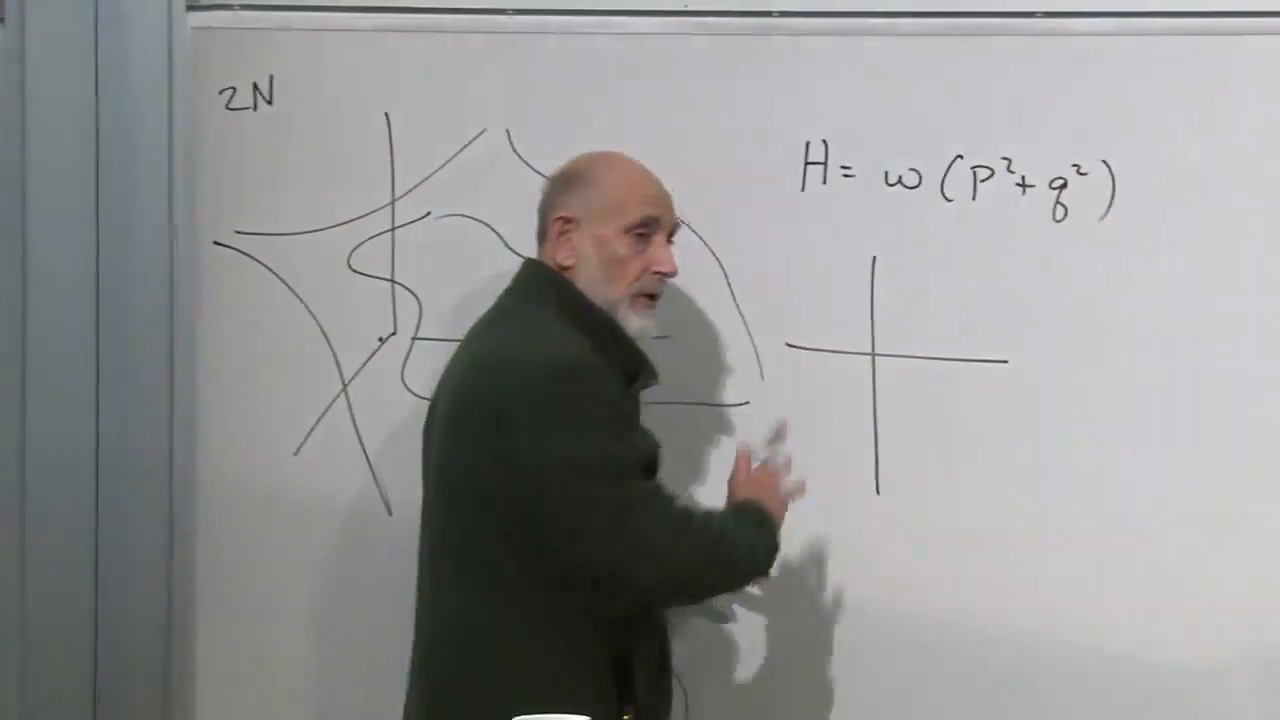
\includegraphics[width=0.84\textwidth]{lecture_07_figure_04.png}
  \caption{用于引入等能面的\(2n\)维相空间示意图和谐振子哈密顿量。}
  \lectureframe{00:15:20}
\end{figure}

运动方程，
\begin{equation}
  \dot q=\omega p,\qquad \dot p=-\omega q,
  \label{eq:l7-oscillator-flow}
\end{equation}
使该点沿其圆顺时针运动。能量方程告诉我们哪条曲线包含该运动；哈密顿方程告诉我们沿该曲线的方向和速率。

\begin{figure}[htbp]
  \centering
  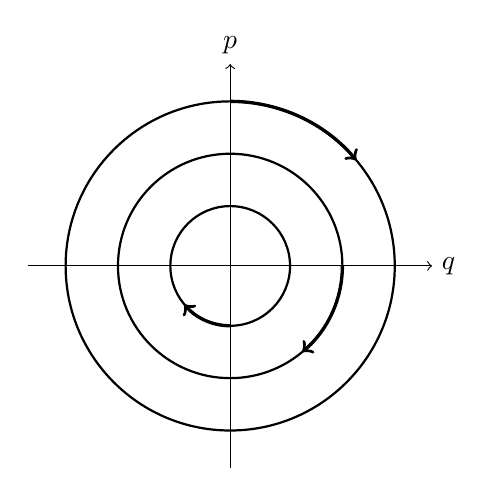
\begin{tikzpicture}[scale=0.95]
    \draw[->] (-2.7,0) -- (2.7,0) node[right] {\(q\)};
    \draw[->] (0,-2.7) -- (0,2.7) node[above] {\(p\)};
    \draw[thick] (0,0) circle (0.8);
    \draw[thick] (0,0) circle (1.5);
    \draw[thick] (0,0) circle (2.2);
    \draw[->,very thick] (0,2.2) arc[start angle=90,end angle=40,radius=2.2];
    \draw[->,very thick] (1.5,0) arc[start angle=0,end angle=-50,radius=1.5];
    \draw[->,very thick] (0,-0.8) arc[start angle=-90,end angle=-140,radius=0.8];
  \end{tikzpicture}
  \caption{等能给出这些圆；振子方程给出顺时针切向流。}
\end{figure}

\begin{classroomqa}
  \audiencequestion{哈密顿的两个方程和\(H=E\)是同一个方程的几种版本吗？
  \lecturetimestamp{00:15:53--00:17:06}}
  \lecturerresponse{不是。哈密顿方程是一个正则对的两个一阶运动定律。它们蕴含\(dH/dt=0\)，由此推出\(H=E\)。\(E\)的值由初始条件选定。方程\(H=E\)标识一个曲面；它本身并不指定沿该曲面的速度。}
\end{classroomqa}

\section{从一个状态到状态的流}

与其追踪一个初始条件，不如在相空间中撒满每一个可能的初始条件，然后启动时钟。每个点都是一个完整的可能状态，而每个状态都按照哈密顿方程运动。这种撒布可以想象为尘埃或一种假想流体。并没有任何物质被倒入相空间；这种流体是一种同时看到所有轨迹的方式。

相空间速度场为
\begin{equation}
  \mathbf V(q,p,t)
  =
  (\dot q_1,\ldots,\dot q_n,\dot p_1,\ldots,\dot p_n).
  \label{eq:l7-phase-velocity}
\end{equation}
对于一个正则对，我们写
\begin{equation}
  V_q=\dot q=\frac{\partial H}{\partial p},
  \qquad
  V_p=\dot p=-\frac{\partial H}{\partial q}.
  \label{eq:l7-phase-components}
\end{equation}
在每一点，哈密顿量赋予一个矢量，告诉相点下一步去哪里。如果\(H\)与时间无关，则矢量场是驻定的：回到同一个相点给出相同的速度。如果\(H\)依赖于时间，则矢量场本身随时间变化，但它在每一瞬间仍然有定义。

\begin{figure}[htbp]
  \centering
  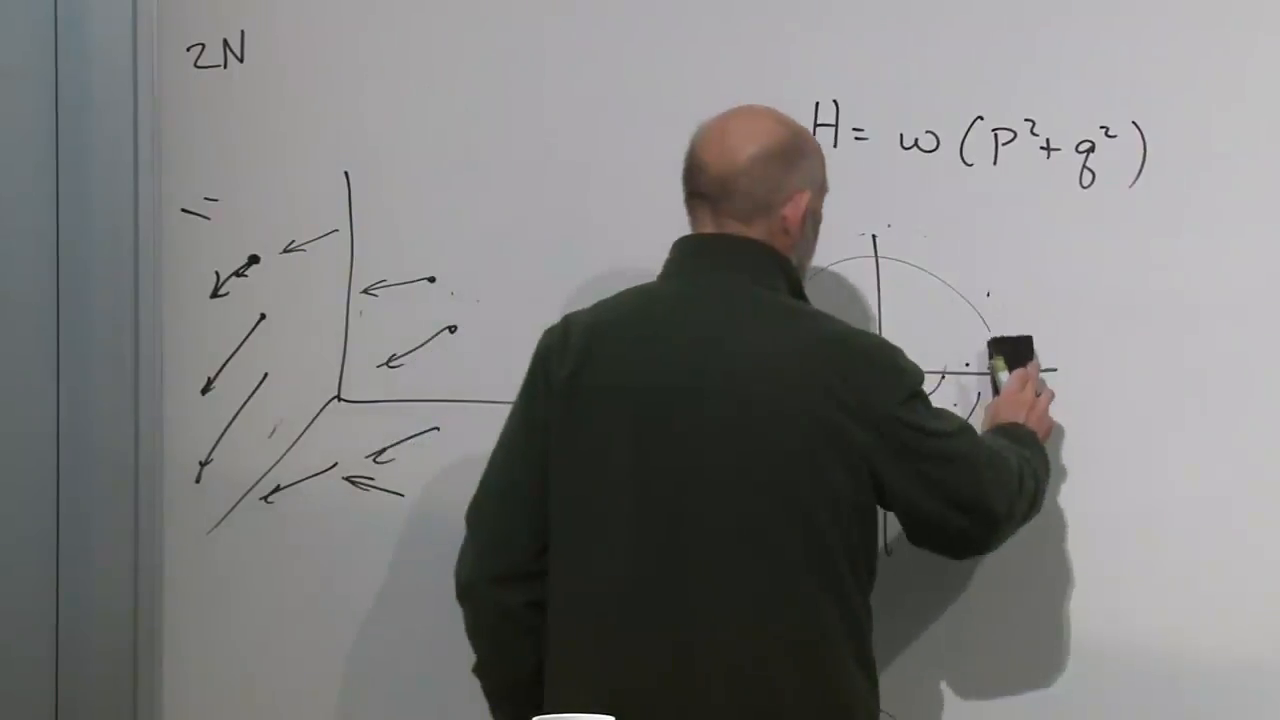
\includegraphics[width=0.84\textwidth]{lecture_07_figure_05.png}
  \caption{谐振子的速度场。这些矢量与圆相切，并且越靠近原点越短。}
  \lectureframe{00:24:50}
\end{figure}

对于谐振子，每个半径都以角速度\(\omega\)转动。靠近原点的点具有较小的线速度，因为它们在相同周期内走过一个更短的圆。因此整团尘埃像一个刚性旋转木马一样旋转。

\begin{classroomqa}
  \audiencequestion{刚体旋转是否意味着所有振子轨迹都具有相同的周期？\lecturetimestamp{00:21:10--00:21:42}}
  \lecturerresponse{是的。这种与振幅无关的性质正是谐振子的定义性特殊属性。每个圆都以相同的角频率\(\omega\)被遍历，尽管在较小的圆上相空间速度的大小较小。}
\end{classroomqa}

\begin{classroomqa}
  \audiencequestion{相空间速度在每一点都相同吗？\lecturetimestamp{00:24:29--00:25:37}}
  \lecturerresponse{不。其方向和大小通常都随位置变化。对于振子，该矢量与局部圆相切，大小为\(\omega\sqrt{p^2+q^2}\)。矢量场意味着在每一点指定一个矢量，而不是把一个相同的矢量复制到各处。}
\end{classroomqa}

\begin{classroomqa}
  \audiencequestion{这种假想流体的粒子和密度究竟是什么？\lecturetimestamp{00:56:03--00:58:40}}
  \lecturerresponse{每一点是整个力学系统的一个完整状态。它不是单个物理粒子。五个在一维空间中运动的粒子需要五个位置和五个动量，因此需要十维相空间；在三维中它们需要三十维。尘埃是备选状态的系综。如果流体的图像令人分心，只需取初始条件的一个区域，演化其中每一点，并比较其相空间体积在演化前后的变化。}
\end{classroomqa}

\section{压缩与散度}

要问这种假想流体是否损失体积，先从一维开始。设直线上的点以速度\(v(x)\)运动。相距\(\delta x\)的两个邻近点具有速度差
\begin{equation}
  \delta v \simeq \frac{dv}{dx}\,\delta x.
  \label{eq:l7-one-dimensional-strain}
\end{equation}
若\(dv/dx>0\)，则前方的点运动更快，间隔被拉伸。若\(dv/dx<0\)，则它被压缩。因此，定常的一维不可压缩流动满足
\begin{equation}
  \frac{dv}{dx}=0.
  \label{eq:l7-one-dimensional-incompressible}
\end{equation}

\begin{figure}[htbp]
  \centering
  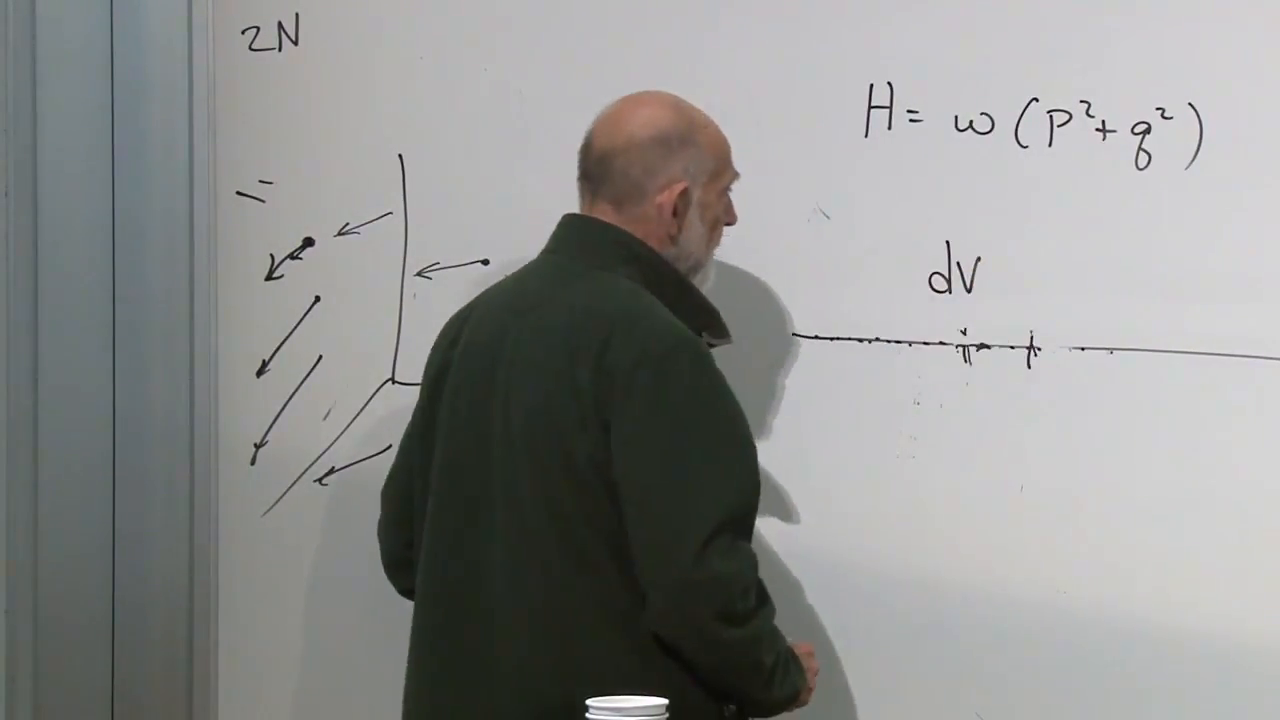
\includegraphics[width=0.84\textwidth]{lecture_07_figure_06.png}
  \caption{导致\(dv/dx\)作为局部拉伸或压缩速率的一维构造。}
  \lectureframe{00:30:20}
\end{figure}

有两种等价的观点。我们可以跟随一个物质间隔，问它的长度是否变化。或者我们可以固定一个小间隔，问单位时间进入的量是否等于离开的量。第一种跟随流体；第二种观察流体经过。

在多于一个维度时，一个区域可以沿一个轴拉伸并沿另一个轴压缩，而总体积不变。对于速度场\(\mathbf V=(V_x,V_y,V_z)\)，相关的局部速率是散度，
\begin{equation}
  \nabla\cdot\mathbf V
  =
  \frac{\partial V_x}{\partial x}
  +\frac{\partial V_y}{\partial y}
  +\frac{\partial V_z}{\partial z}.
  \label{eq:l7-spatial-divergence}
\end{equation}
正散度是局部膨胀，负散度是局部收缩，而不可压缩性为
\begin{equation}
  \nabla\cdot\mathbf V=0.
  \label{eq:l7-zero-divergence}
\end{equation}
通过固定小盒的流入与流出相等，与运动小盒体积保持不变，是同一个局部陈述。

\begin{figure}[htbp]
  \centering
  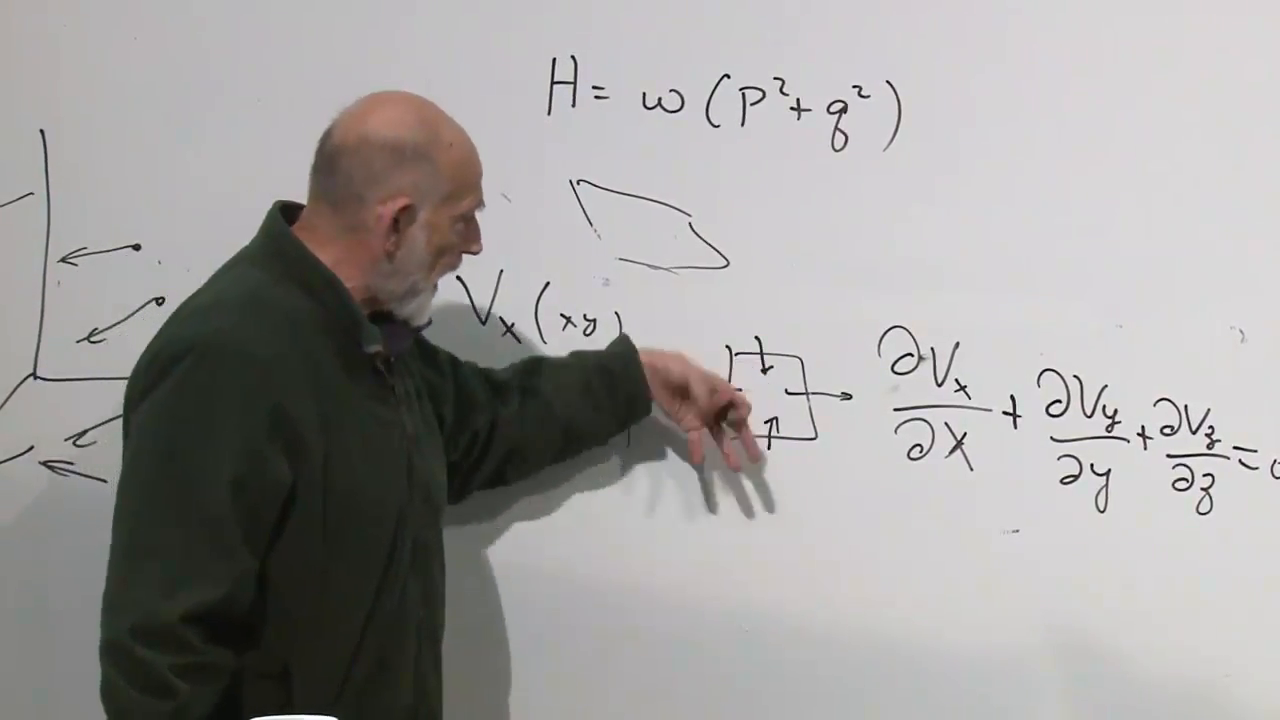
\includegraphics[width=0.86\textwidth]{lecture_07_figure_07.png}
  \caption{一个二维盒、其流动分量，以及定义散度的同坐标导数之和。}
  \lectureframe{00:35:30}
\end{figure}

\begin{classroomqa}
  \audiencequestion{我们讨论的是普通空间中的流体，还是相空间中的流动？\lecturetimestamp{00:34:27--00:34:40}}
  \lecturerresponse{散度论证首先是一个一般的流体论证。我们将把它应用于偶数维相空间，其中坐标方向是\(q_i\)和\(p_i\)，速度分量是\(\dot q_i\)和\(\dot p_i\)。}
\end{classroomqa}

现在回到离散状态映射。在可逆循环中，每个节点都有一条箭头进入和一条箭头离开，并且所选的一组状态在演化过程中保持相同的成员数。而在汇中，许多箭头进入，离开的太少；若干备选状态变得不可区分。

\begin{figure}[htbp]
  \centering
  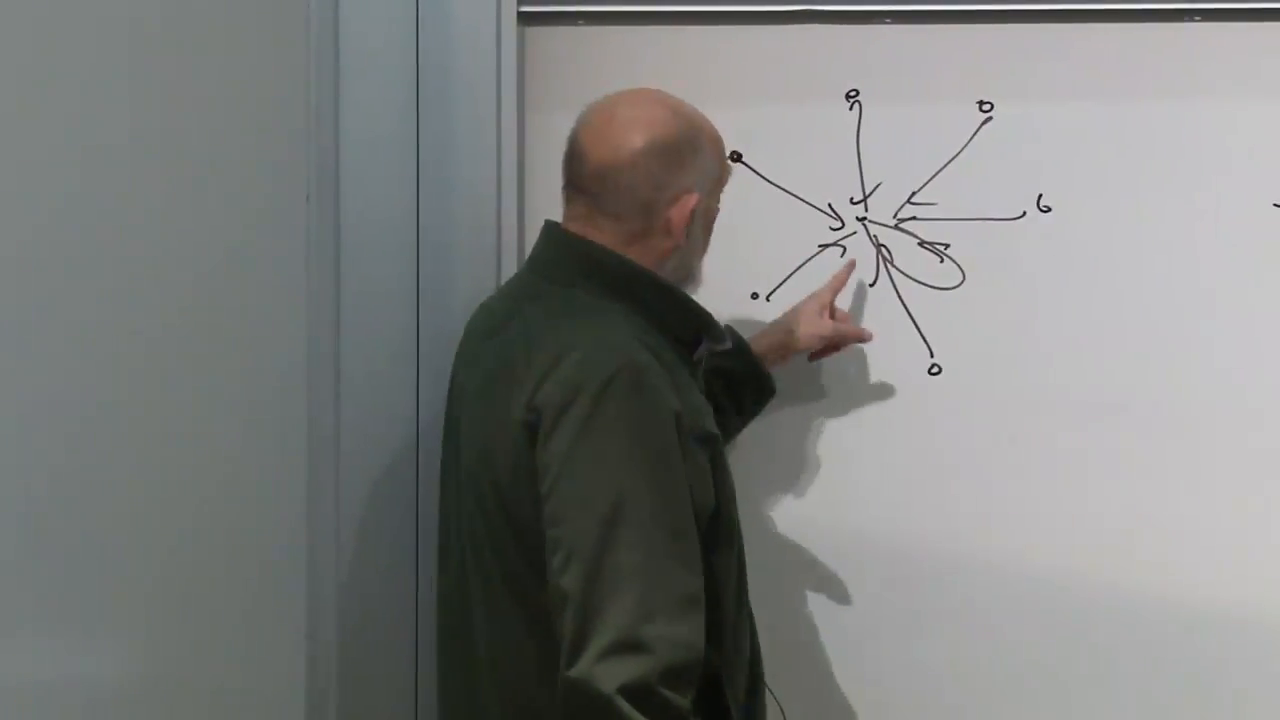
\includegraphics[width=0.80\textwidth]{lecture_07_figure_08.png}
  \caption{用于把散度与第一讲中可逆定律的检验重新联系起来的离散汇。}
  \lectureframe{00:40:15}
\end{figure}

连续的问题现在变得精确：哈密顿流是否具有零散度，从而一小块可区分状态的区域永远不会被压扁成更小的相空间体积？

\section{刘维尔定理}

\begin{theorem}[Liouville's theorem]
对于光滑的哈密顿系统，正则相空间速度场具有零散度：
\begin{equation}
  \sum_i\left(
    \frac{\partial\dot q_i}{\partial q_i}
    +\frac{\partial\dot p_i}{\partial p_i}
  \right)=0.
  \label{eq:l7-liouville-divergence}
\end{equation}
等价地，哈密顿演化保持正则相空间体积\(dq_1\cdots dq_n\,dp_1\cdots dp_n\)。
\end{theorem}

\begin{classroomqa}
  \audiencequestion{被称为\(V\)的分量是否就是\(p\)-点与\(q\)-点？\lecturetimestamp{00:42:20--00:43:22}}
  \lecturerresponse{是的。对于一对，
  \(V_q=\dot q\)和\(V_p=\dot p\)。把所有这样的导数排列起来，就给出完整相空间中流动的速度矢量。}
\end{classroomqa}

对于一对正则变量，哈密顿方程给出
\begin{equation}
  V_p=-\frac{\partial H}{\partial q},
  \qquad
  V_q=\frac{\partial H}{\partial p}.
  \label{eq:l7-liouville-components}
\end{equation}
因此散度为
\begin{align}
  \frac{\partial V_p}{\partial p}
  +\frac{\partial V_q}{\partial q}
  &=
  -\frac{\partial}{\partial p}
    \left(\frac{\partial H}{\partial q}\right)
  +\frac{\partial}{\partial q}
    \left(\frac{\partial H}{\partial p}\right)\\
  &=
  -\frac{\partial^2H}{\partial p\,\partial q}
  +\frac{\partial^2H}{\partial q\,\partial p}
  =0.
  \label{eq:l7-liouville-proof}
\end{align}

\begin{figure}[htbp]
  \centering
  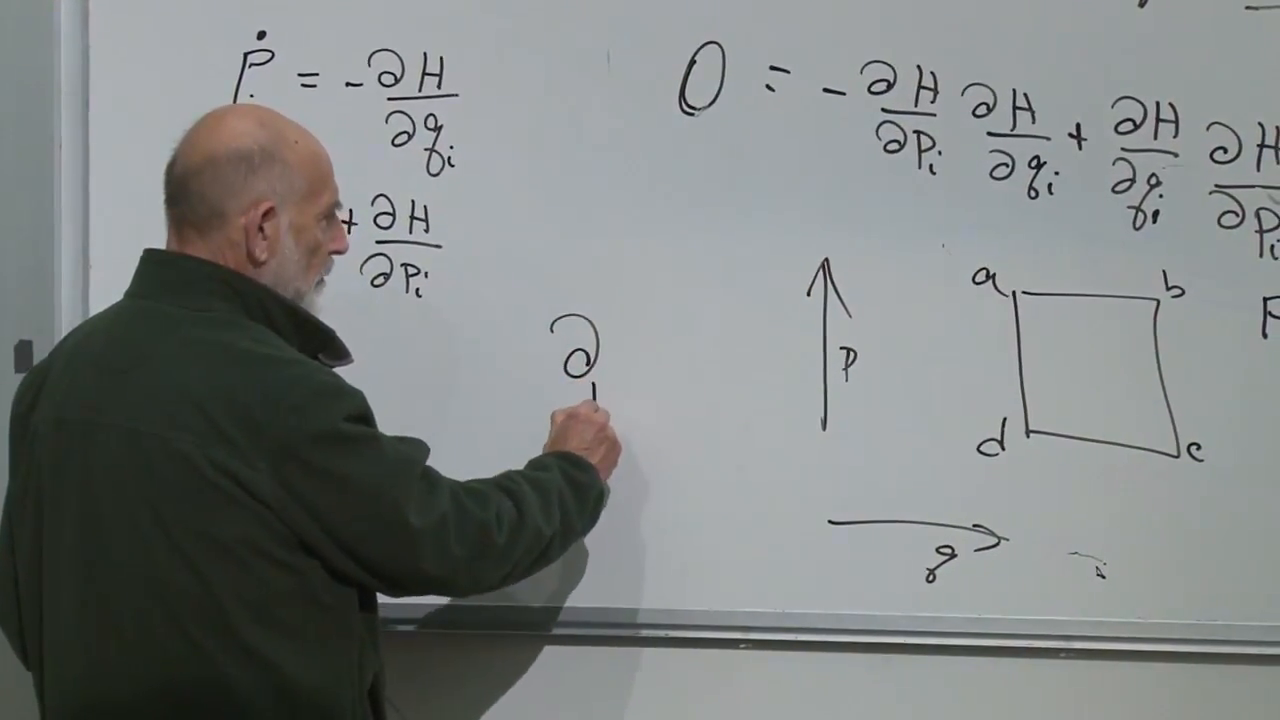
\includegraphics[width=0.86\textwidth]{lecture_07_figure_09.png}
  \caption{用于解释光滑混合偏导数为何可交换的有限差分矩形。}
  \lectureframe{00:47:30}
\end{figure}

混合偏导数的相等性可以通过 \(q\)-\(p\) 平面中一个小矩形角上的四个邻近点 \(A,B,C,D\) 看出。先取 \(q\)-差分再取 \(p\)-差分，除两条小边长外，得到
\begin{equation}
  F(B)+F(D)-F(A)-F(C).
  \label{eq:l7-finite-difference-combination}
\end{equation}
以相反顺序取差分得到相同的组合。在小矩形极限下，只要所需的导数连续，这就是
\(\partial_p\partial_qF=\partial_q\partial_pF\)。

\begin{figure}[htbp]
  \centering
  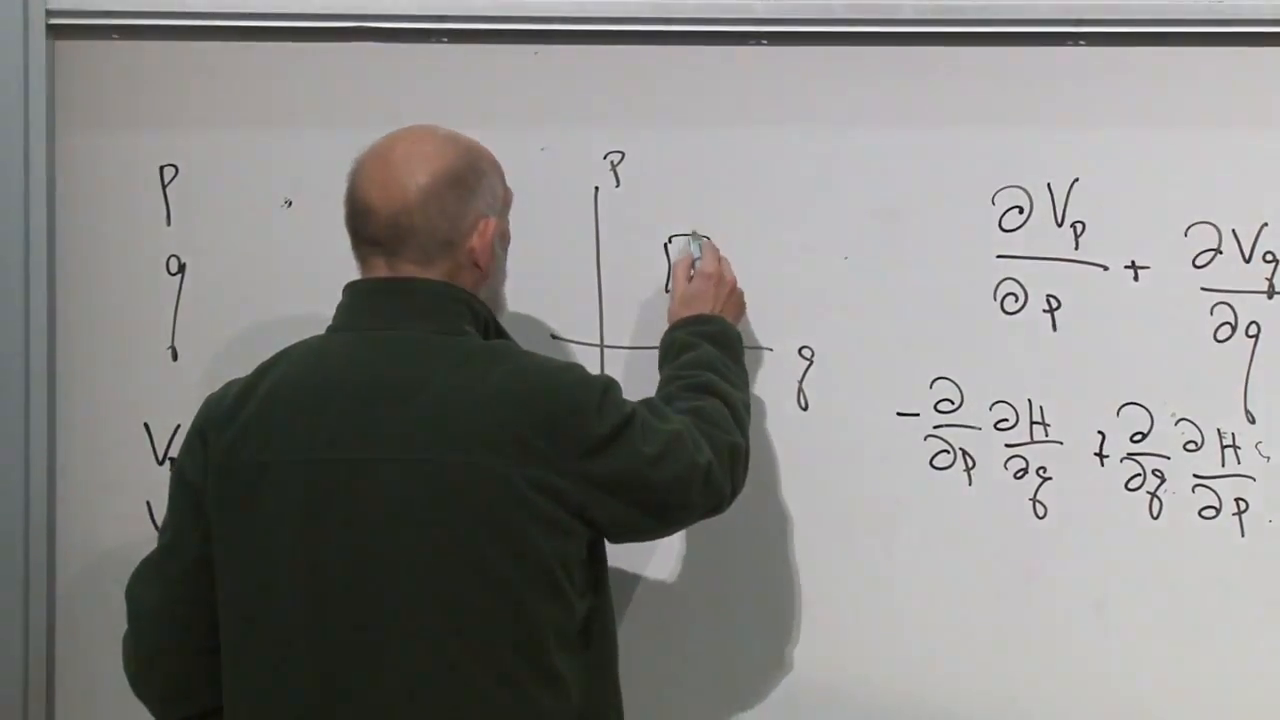
\includegraphics[width=0.88\textwidth]{lecture_07_figure_10.png}
  \caption{哈密顿方程将其约化为两个符号相反的混合导数后的正则散度。}
  \lectureframe{00:50:20}
\end{figure}

对于多个自由度，同样的抵消对每个正则对都发生：
\begin{align}
  \sum_i\left(
    \frac{\partial\dot p_i}{\partial p_i}
    +\frac{\partial\dot q_i}{\partial q_i}
  \right)
  &=
  \sum_i\left(
    -\frac{\partial^2H}{\partial p_i\,\partial q_i}
    +\frac{\partial^2H}{\partial q_i\,\partial p_i}
  \right)\\
  &=0.
  \label{eq:l7-many-pair-proof}
\end{align}
在一个正则方向上的拉伸由其共轭方向上的压缩所平衡。这种成对抵消是比无关轴之间的偶然抵消更强的结构。

\begin{classroomqa}
  \audiencequestion{对所有正则对的求和是否已理解？
  \lecturetimestamp{00:52:00--00:52:36}}
  \lecturerresponse{是的。方程~\eqref{eq:l7-many-pair-proof}对
  \(i\)求和，两个混合导数在每个
  \(q_i,p_i\)对内分别抵消。}
\end{classroomqa}

\begin{classroomqa}
  \audiencequestion{所显示的散度看起来是笛卡尔形式的。该定理在坐标变换下是否仍然成立？
  \lecturetimestamp{00:52:50--00:53:22,\allowbreak\ 00:58:18--00:58:40}}
  \lecturerresponse{自然的陈述是在正则坐标下并借助正则体积元
  \(dq_1\cdots dq_n\,dp_1\cdots dp_n\)作出的。正则变换，或称辛变换，同时改变坐标和动量并保持该体积。在任意的非正则坐标中，体积测度中应包含一个雅可比因子；坐标增量的朴素乘积未必是不变的。}
\end{classroomqa}

\begin{classroomqa}
  \audiencequestion{刘维尔定理是否要求哈密顿量不显含时间？\lecturetimestamp{00:53:43--00:55:51}}
  \lecturerresponse{不要求。能量守恒要求
  \(\partial H/\partial t=0\)，但散度证明只在固定时间下对 \(q_i\) 和 \(p_i\) 求导。对于
  \(H(q,p,t)\)，混合偏导数仍然抵消。因此，含时哈密顿量生成一个含时但在每一瞬时保持体积的正则流。}
\end{classroomqa}

\section{体积保持意味着什么、不意味着什么}

取初始条件的任意小区域 \(R_0\)，将其中每一点演化一段时间 \(t\)。刘维尔定理说
\begin{equation}
  \operatorname{Vol}(R_t)=\operatorname{Vol}(R_0).
  \label{eq:l7-volume-preservation}
\end{equation}
该区域可能移动、旋转、剪切并拉伸成一条长丝。受保护的是它的体积，而不是它的形状。在有限的、光滑的哈密顿演化中，不同的相点不能合并。

对于有限时间，光滑的哈密顿流是一个可逆映射，其光滑逆映射通过向后演化得到。这也解释了课堂上的说法：一个连通的团块不能收缩成不连通的部分：该流连续地变形该区域并保持其拓扑，尽管极细的颈部可能使两个瓣在有限分辨率下看起来是分开的。

\begin{figure}[htbp]
  \centering
  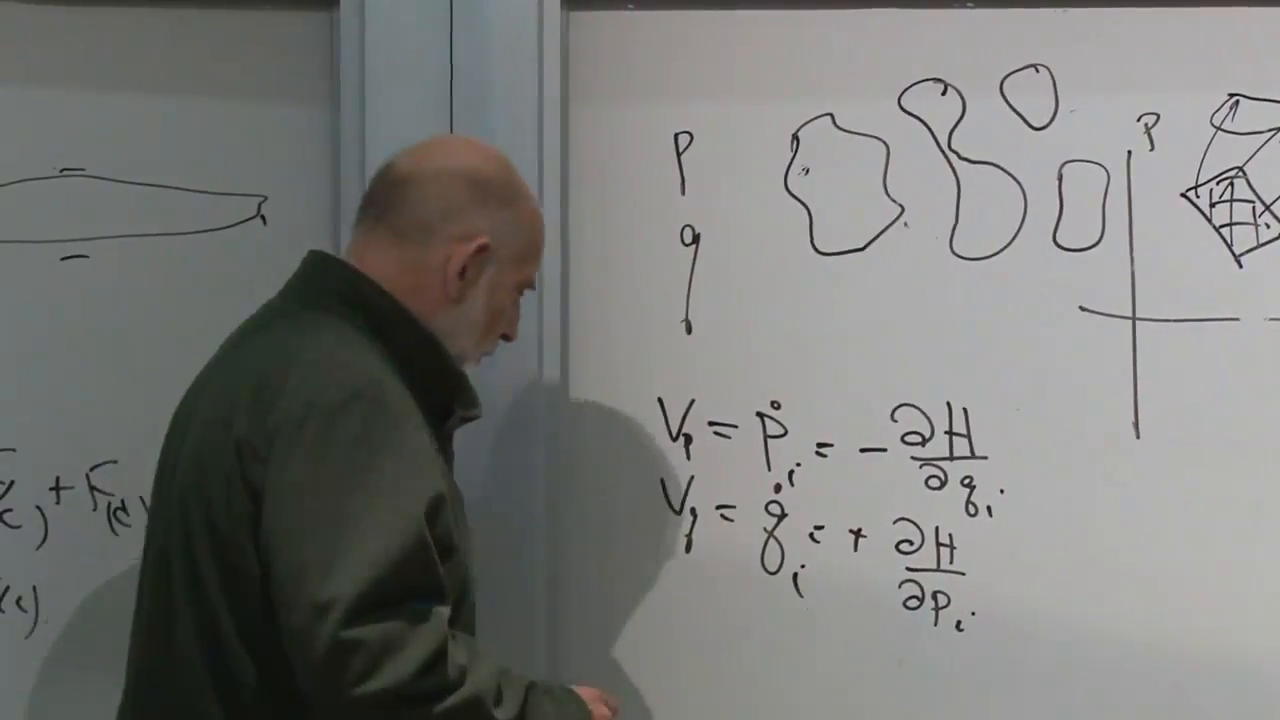
\includegraphics[width=0.86\textwidth]{lecture_07_figure_12.png}
  \caption{一个相空间区域的可能变形。光滑的哈密顿流可能产生细颈，但不会在有限时间内真正断裂成独立演化的部分。}
  \lectureframe{01:04:55}
\end{figure}

\begin{classroomqa}
  \audiencequestion{相空间区域能否收缩断开并分裂成两部分？\lecturetimestamp{01:04:10--01:05:49}}
  \lecturerresponse{在有限时间的光滑确定性哈密顿流下不能。在假想的收缩点处仍然只有一个相空间点和一个被赋予的速度，而不是两个不相容的方向。该区域可以发展出一条非常长而狭窄的连接细丝，但演化仍然是一一对应的，不会将其撕裂。}
\end{classroomqa}

\begin{classroomqa}
  \audiencequestion{被拉伸团块的两个相距很远的部分在物理上是连接的，还是量子纠缠的？
  \lecturetimestamp{01:08:01--01:09:16}}
  \lecturerresponse{并不蕴含这样的物理连接。该团块是一组备选初始条件，而不是一个物质客体。称其为一个区域记录的是这些态所演化自的共同集合；它并未说明它们之间的力或量子纠缠。}
\end{classroomqa}

\begin{classroomqa}
  \audiencequestion{刚性摆的竖直不稳定平衡附近会发生什么？顺时针和逆时针的轨迹会重叠吗？
  \lecturetimestamp{01:07:07--01:07:47}}
  \lecturerresponse{邻近的初始条件可以分离到非常不同的轨迹上，从而产生刚才描述的细丝。它们不会变成同一个相点：无穷小位移或动量的符号区分了两侧。完全平衡的状态有其自身唯一确定的运动，即在理想模型中保持在平衡态。}
\end{classroomqa}

\subsection{位置空间中的膨胀与动量空间中的收缩}

若一个正则变换将位置的范围扩大因子\(a\)，则共轭动量的尺度按倒数因子收缩：
\begin{equation}
  q\longrightarrow aq,
  \qquad
  p\longrightarrow \frac{p}{a},
  \qquad
  dq\,dp\longrightarrow dq\,dp.
  \label{eq:l7-canonical-scaling}
\end{equation}
这就是气体膨胀例子背后清晰的相空间内容。在绝热膨胀中，可及的普通空间区域增大，而典型动量下降，气体冷却。详细的热力学关系取决于维度、膨胀协议和相互作用；刘维尔定理提供的是体积约束，而不是每一个热力学系数。

\begin{classroomqa}
  \audiencequestion{同样的推理是否适用于膨胀的宇宙，即使是突然的膨胀？\lecturetimestamp{00:53:23--00:56:00}}
  \lecturerresponse{只要完整的动力学是哈密顿的，刘维尔定理就适用，包括显含时间的正则变量。位置方向上的膨胀必须伴随正则动量方向上相应的收缩。然而，宇宙学标度因子、受控的气体膨胀和自由爆炸的云并不是相同的物理过程。距离与退行速率之间类似哈勃的相关性之所以出现，是因为更快的物体运动得更远，而绝热冷却涉及局部动量分布的收缩。无论哪种情况，该定理都约束完整的相空间映射。}
\end{classroomqa}

\begin{classroomqa}
  \audiencequestion{刘维尔定理有什么实际用途？
  \lecturetimestamp{01:06:16--01:07:04}}
  \lecturerresponse{它是统计力学的核心。它控制微观态系综如何演化，并构成相空间体积与熵之间关系的基础。气体的膨胀和冷却是其中一个直接的例证；后来它成为平衡态和非平衡态推理的基本工具。}
\end{classroomqa}

\section{一种剧烈改变形状的流}

谐振子既保持面积又保持形状，因为它的流是刚性旋转。这是例外情况。为了将体积保持与刚性区分开来，取
\begin{equation}
  H=\lambda pq,
  \label{eq:l7-pq-hamiltonian}
\end{equation}
其中\(\lambda\)具有时间的倒数量纲。讲义设定\(\lambda=1\)；保留它使量纲显式可见。

\begin{figure}[htbp]
  \centering
  \includegraphics[width=0.82\textwidth]{lecture_07_figure_03.png}
  \caption{\(H=pq\)例子的开始以及第一个相空间速度分量。}
  \lectureframe{01:00:11}
\end{figure}

哈密顿方程为
\begin{equation}
  \dot p=-\lambda p,
  \qquad
  \dot q=\lambda q,
  \label{eq:l7-pq-flow}
\end{equation}
其解为
\begin{equation}
  p(t)=p_0e^{-\lambda t},
  \qquad
  q(t)=q_0e^{\lambda t}.
  \label{eq:l7-pq-solutions}
\end{equation}
一个方形小块在\(p\)方向上被指数压缩，并在\(q\)方向上被同一因子拉伸：
\begin{equation}
  \Delta p(t)\Delta q(t)
  =
  \Delta p(0)\Delta q(0).
  \label{eq:l7-pq-area}
\end{equation}
其散度在局部验证了该结果，
\begin{equation}
  \frac{\partial\dot p}{\partial p}
  +\frac{\partial\dot q}{\partial q}
  =-\lambda+\lambda=0.
  \label{eq:l7-pq-divergence}
\end{equation}

\begin{figure}[htbp]
  \centering
  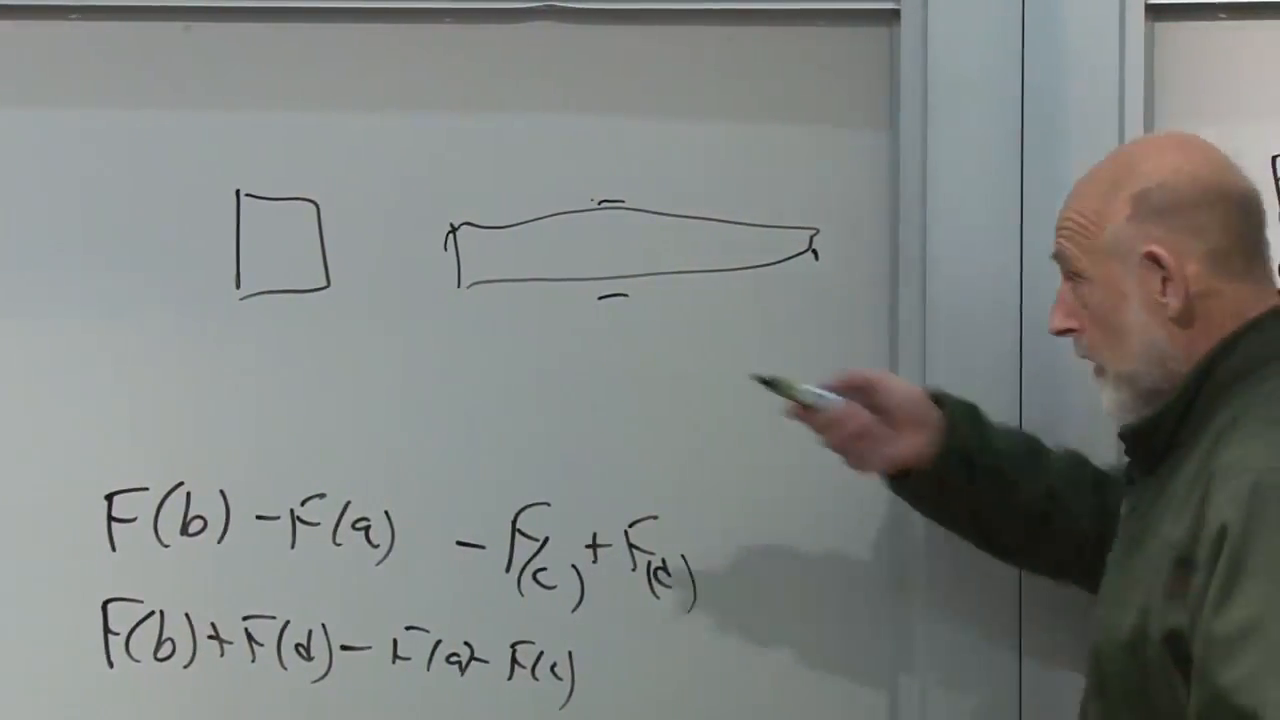
\includegraphics[width=0.86\textwidth]{lecture_07_figure_11.png}
  \caption{在\(H=pq\)流下，一个紧致小块被拉伸成长而薄的条带，同时保持面积。}
  \lectureframe{01:02:10}
\end{figure}

\begin{classroomqa}
  \audiencequestion{既然\(pq\)具有作用量的量纲，刘维尔定理是作用量守恒吗？\lecturetimestamp{01:03:00--01:04:09}}
  \lecturerresponse{不是。该定理守恒的是相空间体积。在一对正则变量中，\(dq\,dp\)具有作用量的量纲，这一量纲事实预示了量子力学，其中相空间元胞以\(\hbar\)设定的单位来度量。但乘积\(pq\)本身并不是哈密顿作用量泛函，也不能仅仅因为量纲一致就自动成为角动量。}
\end{classroomqa}

这个例子还表明角度不必被保持。在式~\eqref{eq:l7-pq-solutions}中的缩放下一个分量不等的直角十字在其度量外观上被剪切，而面积保持不变。刘维尔定理是面积或体积定理，而不是普通的欧几里得刚性定理。

\section{阻尼产生一个汇}

为了看清该定理排除了什么，考虑阻尼振子的约化方程，
\begin{equation}
  m\ddot x=-kx-c\dot x,
  \qquad c>0.
  \label{eq:l7-damped-newton}
\end{equation}
令\(p=m\dot x\)。则
\begin{equation}
  \dot x=\frac{p}{m},
  \qquad
  \dot p=-kx-\frac{c}{m}p.
  \label{eq:l7-damped-first-order}
\end{equation}
没有阻尼时，相点绕原点作圆周运动。有阻尼时，能量被转移到周围介质的微观自由度中，轨道向内螺旋。

\begin{figure}[htbp]
  \centering
  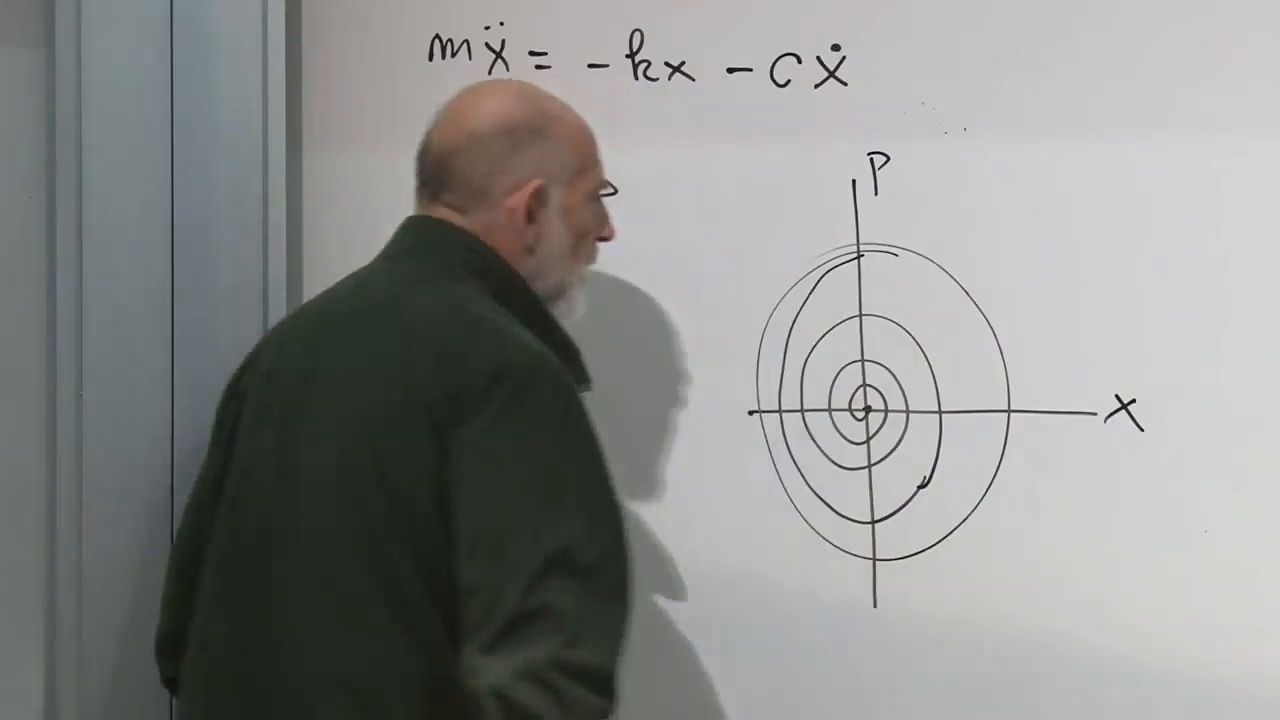
\includegraphics[width=0.84\textwidth]{lecture_07_figure_13.png}
  \caption{阻尼振子方程及其在\(x\)-\(p\)平面上的向内螺旋。}
  \lectureframe{01:13:30}
\end{figure}

这个约化后的二维流动的散度为
\begin{equation}
  \frac{\partial\dot x}{\partial x}
  +\frac{\partial\dot p}{\partial p}
  =
  0-\frac{c}{m}<0.
  \label{eq:l7-damped-divergence}
\end{equation}
每个有限小块都会收缩。原点是汇，即“多箭头汇入”状态映射的连续类比。

\begin{figure}[htbp]
  \centering
  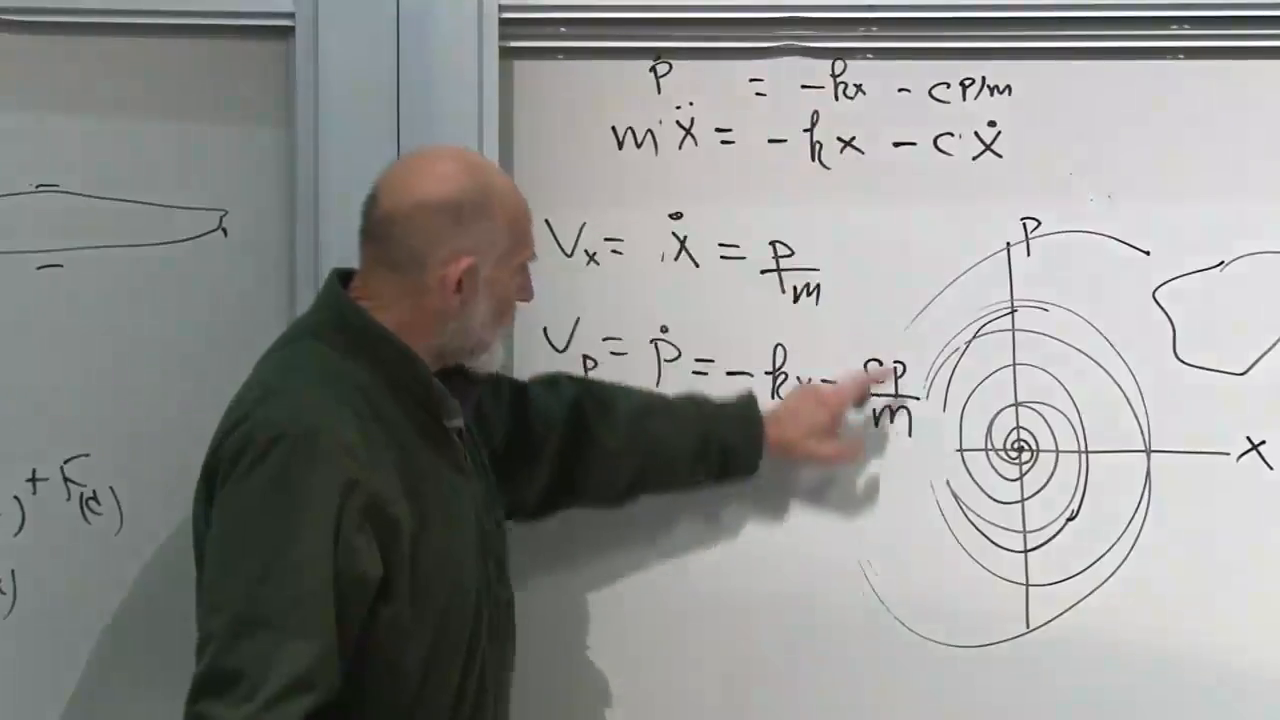
\includegraphics[width=0.88\textwidth]{lecture_07_figure_14.png}
  \caption{用于得到负散度\(-c/m\)的阻尼相空间速度分量。}
  \lectureframe{01:16:05}
\end{figure}

这并不意味着微观力学违反了刘维尔定理。两个变量\(x,p\)省略了接收振子能量的巨量环境自由度。即便其约化后的\(x,p\)描述会收缩，扩大后的振子加环境系统仍可以是哈密顿的且保体积的。

\begin{classroomqa}
  \audiencequestion{尽管阻尼振子在这个约化相空间中不是哈密顿的，它是否仍由牛顿方程描述？
  \lecturetimestamp{01:20:09--01:21:12}}
  \lecturerresponse{是的。牛顿的\(F=ma\)可以包含一个经验给出的阻力。初等的\(L=T-V\)和哈密顿描述直接适用于保守力，而更一般的拉格朗日量也能处理某些依赖于速度的力。然而，对于孤立的一对\(x,p\)而言，马尔可夫摩擦项是约化的耗散动力学，而不是封闭的正则哈密顿系统。}
\end{classroomqa}

\begin{classroomqa}
  \audiencequestion{如果阻尼方程能以无限精度反向积分，信息真的丢失了吗？
  \lecturetimestamp{01:25:16--01:27:17}}
  \lecturerresponse{对于任何有限时间，理想的微分方程仍有逆，因此精确数据可以反向演化。准确的陈述是：有限相空间胞元会指数收缩。于是，恢复它们的过去需要指数增长的精度，而在无限时间时所有轨迹都趋近于汇。这是离散的“选项丢失”图景最接近的连续经典类比，而不是断言两个精确的有限时间解真的变成了一个。}
\end{classroomqa}

\begin{classroomqa}
  \audiencequestion{一个向量场能否具有零散度而不来自哈密顿量？\lecturetimestamp{01:18:21--01:22:34}}
  \lecturerresponse{当然可以。哈密顿形式是零散度的充分条件，而非必要条件。任意的不可压缩速度场可以具有零散度，而不必是同一空间上的正则哈密顿场。三维不可压缩流体速度场就是课堂上的例子：三个坐标本身不能构成正则对。完整的流体力学可能拥有更复杂的无限维哈密顿表述，但这并不能逆转这里所作的单向蕴含。}
\end{classroomqa}

\section{问题所揭示的进一步区分}

\begin{classroomqa}
  \audiencequestion{等能面上的运动与整个相空间体积的保持有何关系？
  \lecturetimestamp{01:28:47--01:30:41}}
  \lecturerresponse{它们是哈密顿结构的独立推论。如果\(H\)不显含时间，每条轨迹都停留在各自的能面上。一个有限小块可能穿过许多这样的能面；刘维尔定理说整个小块的体积保持不变。对于谐振子，小块还保持其形状，因为流动是刚性旋转。而\(H=pq\)小块只保持其面积，不保持其形状。}
\end{classroomqa}

\begin{classroomqa}
  \audiencequestion{机械功在哈密顿描述中处于什么位置？\lecturetimestamp{01:30:44--01:32:57}}
  \lecturerresponse{功描述的是穿过所选系统边界传递的能量。外部作用者可以举起重物或改变参数，从而改变子系统的能量；它提供的能量由该作用者失去。如果双方都包含在一个封闭模型中，重点就回到总能量守恒以及子系统之间的交换。}
\end{classroomqa}

\begin{classroomqa}
  \audiencequestion{保体积是否也保持拓扑和角度？\lecturetimestamp{01:33:00--01:33:37}}
  \lecturerresponse{光滑的有限时间哈密顿流保持拓扑，因为它是可逆的连续形变。它一般不保持欧几里得角度或形状。谐振子的刚性旋转确实保持，但\(H=pq\)的拉伸表明为什么那是一个特例。}
\end{classroomqa}

\begin{classroomqa}
  \audiencequestion{勒让德变换被省略，是因为它没有物理意义吗？\lecturetimestamp{01:33:43--01:34:48}}
  \lecturerresponse{不是。它是有用的变换，把速度描述换成动量描述，并在映射为正则时给出\(H=\sum_i p_i\dot q_i-L\)。即便没有强调其正式名称，这一构造也已被反复使用；只是对于当前的定理而言，并不需要详细的一般理论。}
\end{classroomqa}

\section{泊松括号：下一次压缩}

最后几分钟回到历史主题。十九世纪的力学反复寻找紧凑的结构，把表面上不同的系统联系起来---力学与几何光学、粒子与射线、经典轨迹与波状描述。泊松括号是另一种这样的结构，它们在量子力学中变得尤为重要。

设\(F(q,p)\)为相空间上的任意函数。它可能是一个坐标、一个动量、乘积\(qp\)，或角动量。沿着运动，\begin{equation}
  \frac{dF}{dt}
  =
  \sum_i\left(
    \frac{\partial F}{\partial q_i}\dot q_i
    +\frac{\partial F}{\partial p_i}\dot p_i
  \right).
  \label{eq:l7-f-time-derivative}
\end{equation}
代入哈密顿方程：
\begin{equation}
  \frac{dF}{dt}
  =
  \sum_i\left(
    \frac{\partial F}{\partial q_i}
    \frac{\partial H}{\partial p_i}
    -
    \frac{\partial F}{\partial p_i}
    \frac{\partial H}{\partial q_i}
  \right).
  \label{eq:l7-f-hamiltonian-derivative}
\end{equation}

\begin{figure}[htbp]
  \centering
  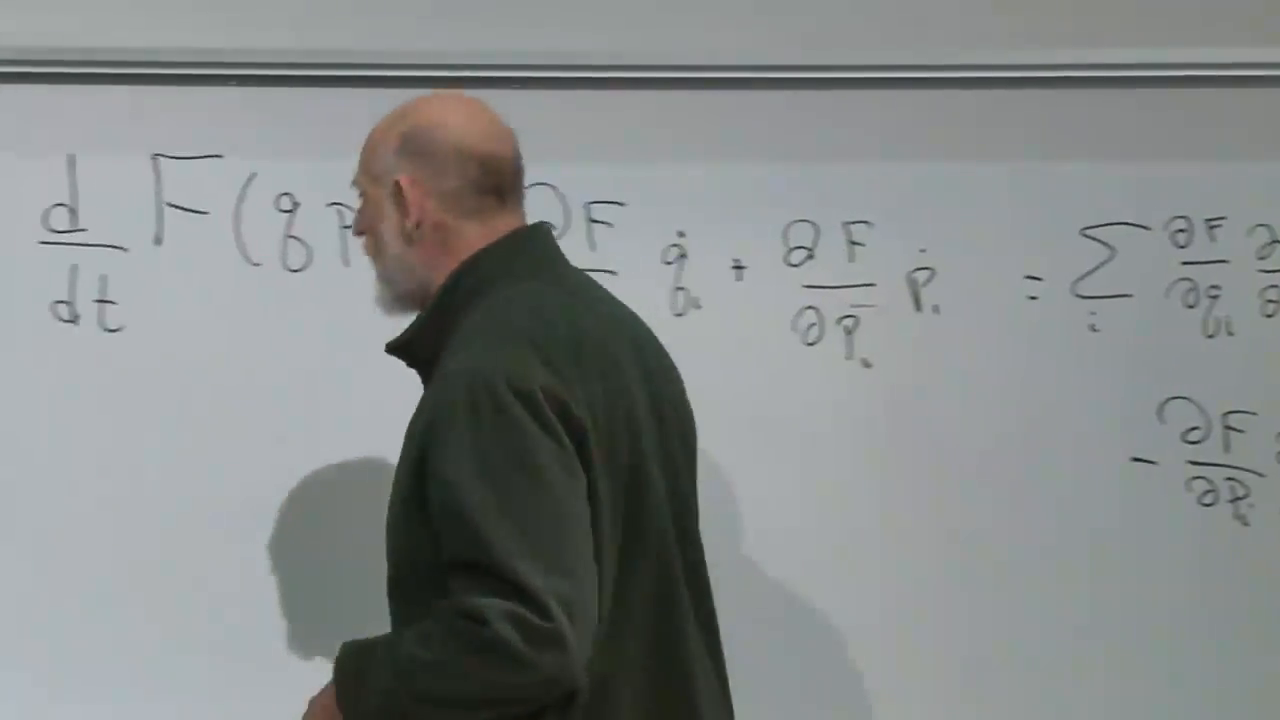
\includegraphics[width=0.88\textwidth]{lecture_07_figure_15.png}
  \caption{一般相空间函数\(F(q,p)\)的时间导数的链式法则。}
  \lectureframe{01:42:40}
\end{figure}

这个反复出现的反对称组合值得一个名称。对于任意两个函数\(F\)和\(G\)，定义它们的泊松括号为
\begin{equation}
  \boxed{
  \{F,G\}
  =
  \sum_i\left(
    \frac{\partial F}{\partial q_i}
    \frac{\partial G}{\partial p_i}
    -
    \frac{\partial F}{\partial p_i}
    \frac{\partial G}{\partial q_i}
  \right).}
  \label{eq:l7-poisson-bracket}
\end{equation}

\begin{figure}[htbp]
  \centering
  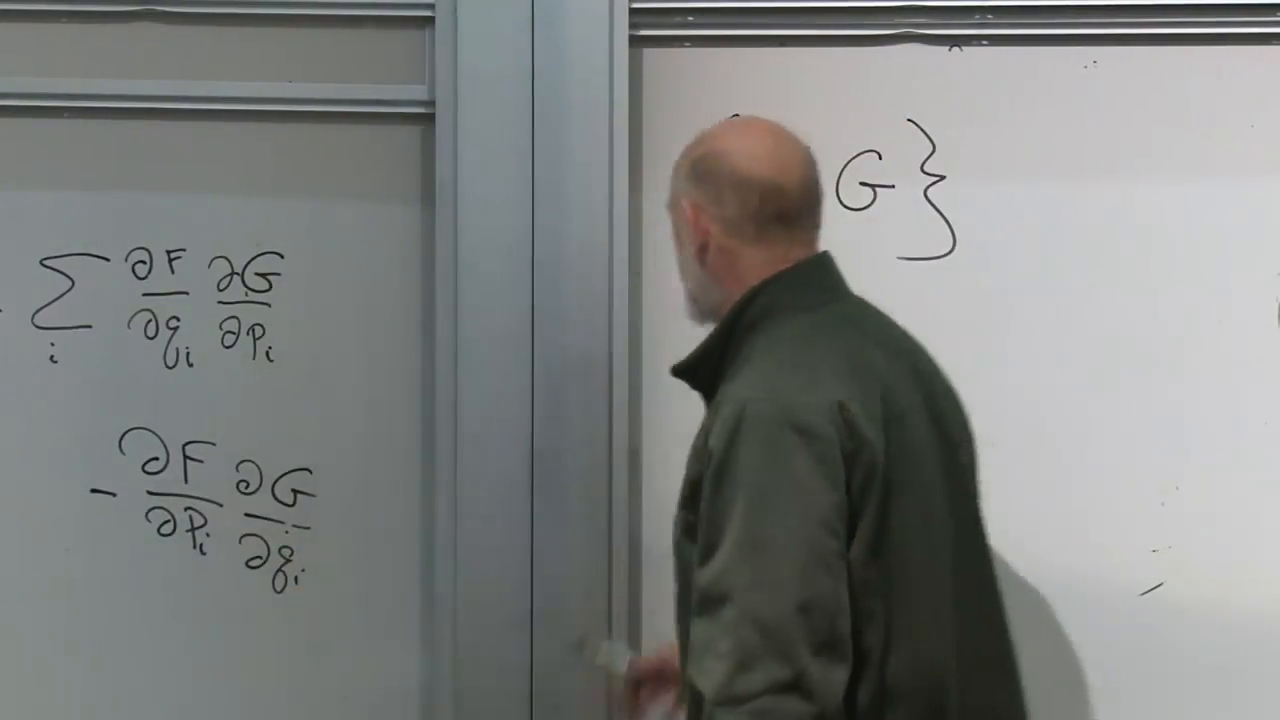
\includegraphics[width=0.86\textwidth]{lecture_07_figure_16.png}
  \caption{双函数导数组合被提升为泊松括号。}
  \lectureframe{01:44:15}
\end{figure}

方程~\eqref{eq:l7-f-hamiltonian-derivative}变为
\begin{equation}
  \boxed{\frac{dF}{dt}=\{F,H\}.}
  \label{eq:l7-hamiltonian-poisson-evolution}
\end{equation}
如果\(F\)还显式依赖于时间，则加上\(\partial F/\partial t\)。取\(F=q_i\)或\(F=p_i\)可恢复哈密顿的两个方程，因此式~\eqref{eq:l7-hamiltonian-poisson-evolution}是完整动力学的一种紧凑形式。

记号总是可以人为地压缩---人们可以把许多方程平方、相加，然后把结果称为一个方程。那会隐藏而不是揭示结构。泊松括号之所以有用，原因恰恰相反：它的代数组织时间演化、守恒量和对称性。下一步是发展这套代数，然后用它处理角动量，其结构在经典力学和量子理论中都将处于核心地位。

\section{可逆性的连续含义}

我们现在可以不加缩短地陈述这一思想链条。当哈密顿量没有显式时间依赖时，哈密顿方程守恒\(H\)，因此个别轨迹保持在等能超曲面上。同一组方程给相空间的每一点指定一个速度。该速度的散度为零，因为混合偏导数两两相消。因此，一整块可能状态的区域保持其正则体积。

这就是一进一出的连续版本。形状可以改变，角度可以改变，相邻轨迹可以极其剧烈地分离。在光滑闭合的哈密顿描述中不可能发生的是，把有限多个备选状态压缩进更小的相空间体积。\(H=pq\)流展示了拉伸的自由；约化阻尼振子展示了一旦放弃哈密顿条件就出现的汇。随后，泊松括号把同一动力学浓缩为这样一个陈述：哈密顿量生成每一个时间导数。